\chapter{GP-EKF example scenarios}\label{chap:gp_ekf_examples}
This chapter contains several hand-picked scenarios for the GP-EKF from statistical testing in \cref{chap:stat_testing}.
The legends and descriptions are omitted from the figures, but all figures follow the same pattern. Red corresponds to the prediction, blue is the training data, and yellow is the ground truth. The ellipses show the $95\%$ CI. Each whole page figure includes the prediction from the basic GP-EKF, GP-EKF with \acrshort{cog} data, GP-EKF with \acrshort{pdaf} and GP-EKF with \acrshort{sl} update.

\begin{figure}
    \begin{subfigure}{\textwidth}
        \makebox[\textwidth][c] {
            \begin{subfigure}{.65\textwidth}
                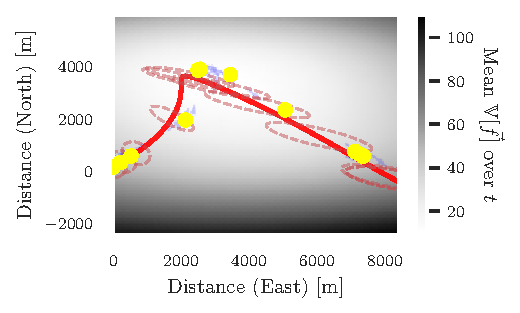
\includegraphics{figures/curved_examples/run_5_pos_no_pdaf.pdf}
            \end{subfigure}
            \begin{subfigure}{.60\textwidth}
                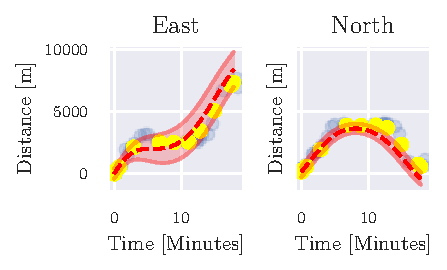
\includegraphics{figures/curved_examples/run_5_state_no_pdaf.pdf}
            \end{subfigure}
        }
        \caption{Basic GP-EKF}
    \end{subfigure}
    \begin{subfigure}{\textwidth}

        \makebox[\textwidth][c] {
            \begin{subfigure}{.65\textwidth}
                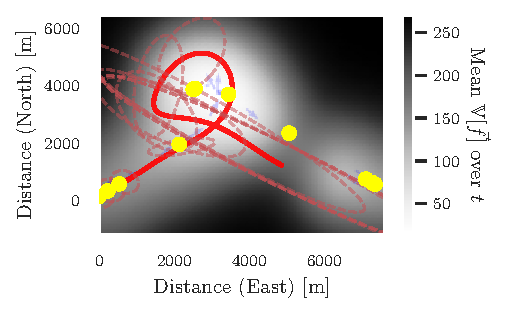
\includegraphics{figures/curved_examples/run_5_pos_no_pdaf_cog.pdf}
            \end{subfigure}
            \begin{subfigure}{.60\textwidth}
                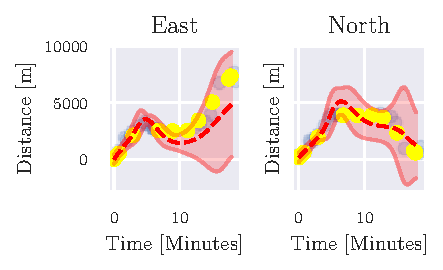
\includegraphics{figures/curved_examples/run_5_state_no_pdaf_cog.pdf}
            \end{subfigure}
        }
        \caption{GP-EKF using \acrshort{cog} / \acrshort{sog} data}
    \end{subfigure}

    \begin{subfigure}{\textwidth}
        \makebox[\textwidth][c] {
            \begin{subfigure}{.65\textwidth}
                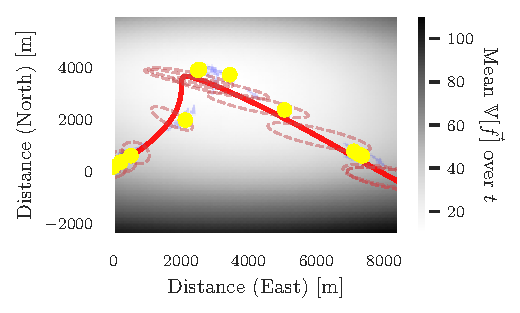
\includegraphics{figures/curved_examples/run_5_pos_pdaf.pdf}
            \end{subfigure}
            \begin{subfigure}{.60\textwidth}
                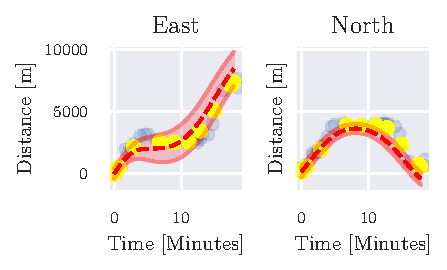
\includegraphics{figures/curved_examples/run_5_state_pdaf.pdf}
            \end{subfigure}
        }
        \caption{GP-EKF With PDAF update}
    \end{subfigure}

    \begin{subfigure}{\textwidth}
        \makebox[\textwidth][c] {
            \begin{subfigure}{.65\textwidth}
                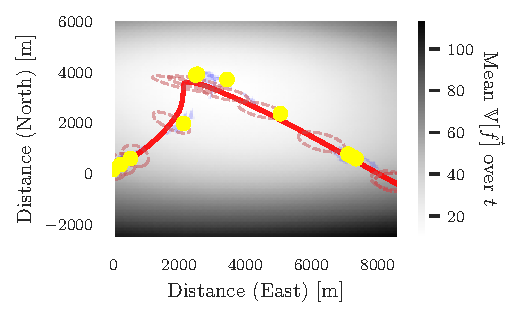
\includegraphics{figures/curved_examples/run_5_pos_syn.pdf}
            \end{subfigure}
            \begin{subfigure}{.60\textwidth}
                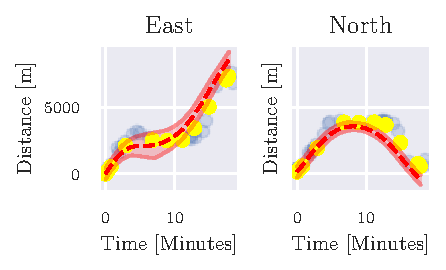
\includegraphics{figures/curved_examples/run_5_state_syn.pdf}
            \end{subfigure}
        }
        \caption{GP-EKF with \acrshort{sl} update}
    \end{subfigure}
    \caption{Case 1}
\end{figure}

\begin{figure}
    \begin{subfigure}{\textwidth}
        \makebox[\textwidth][c] {
            \begin{subfigure}{.65\textwidth}
                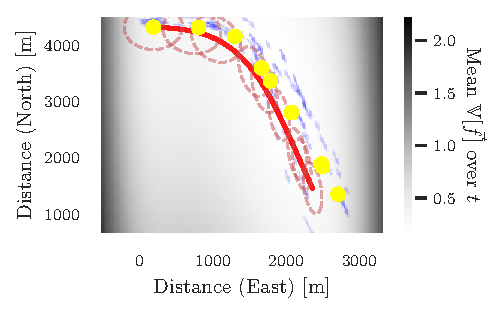
\includegraphics{figures/curved_examples/run_13_pos_no_pdaf.pdf}
            \end{subfigure}
            \begin{subfigure}{.60\textwidth}
                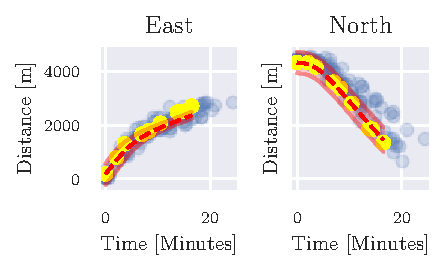
\includegraphics{figures/curved_examples/run_13_state_no_pdaf.pdf}
            \end{subfigure}
        }
        \caption{Basic GP-EKF}
    \end{subfigure}
    \begin{subfigure}{\textwidth}

        \makebox[\textwidth][c] {
            \begin{subfigure}{.65\textwidth}
                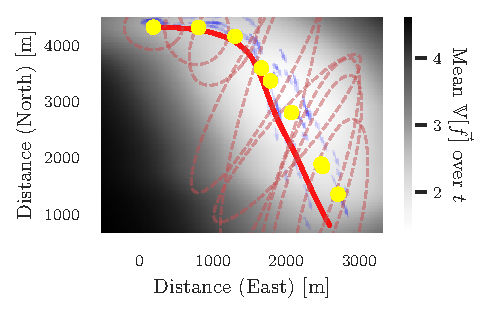
\includegraphics{figures/curved_examples/run_13_pos_no_pdaf_cog.pdf}
            \end{subfigure}
            \begin{subfigure}{.60\textwidth}
                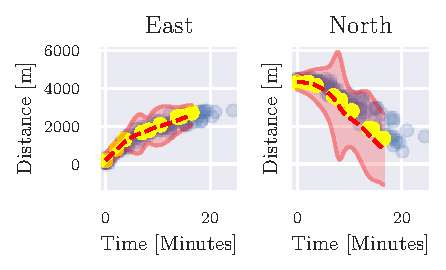
\includegraphics{figures/curved_examples/run_13_state_no_pdaf_cog.pdf}
            \end{subfigure}
        }
        \caption{GP-EKF using \acrshort{cog} / \acrshort{sog} data}
    \end{subfigure}

    \begin{subfigure}{\textwidth}
        \makebox[\textwidth][c] {
            \begin{subfigure}{.65\textwidth}
                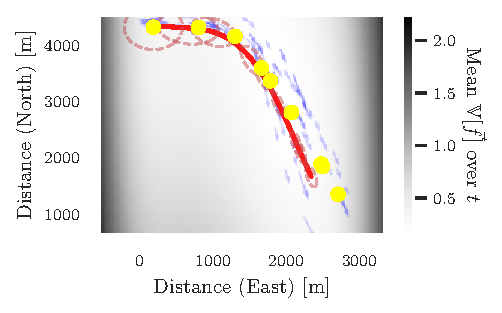
\includegraphics{figures/curved_examples/run_13_pos_pdaf.pdf}
            \end{subfigure}
            \begin{subfigure}{.60\textwidth}
                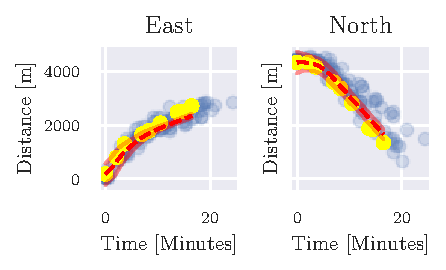
\includegraphics{figures/curved_examples/run_13_state_pdaf.pdf}
            \end{subfigure}
        }
        \caption{GP-EKF With PDAF update}
    \end{subfigure}

    \begin{subfigure}{\textwidth}
        \makebox[\textwidth][c] {
            \begin{subfigure}{.65\textwidth}
                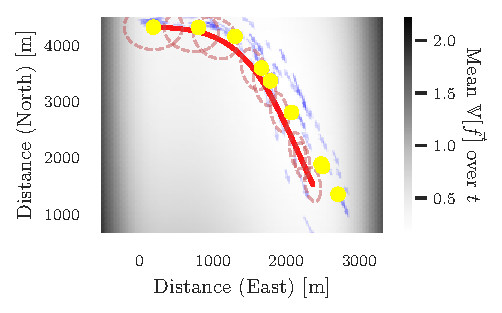
\includegraphics{figures/curved_examples/run_13_pos_syn.pdf}
            \end{subfigure}
            \begin{subfigure}{.60\textwidth}
                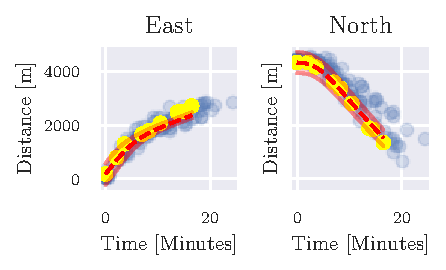
\includegraphics{figures/curved_examples/run_13_state_syn.pdf}
            \end{subfigure}
        }
        \caption{GP-EKF with \acrshort{sl} update}
    \end{subfigure}
    \caption{Case 2}
\end{figure}

\begin{figure}
    \begin{subfigure}{\textwidth}
        \makebox[\textwidth][c] {
            \begin{subfigure}{.65\textwidth}
                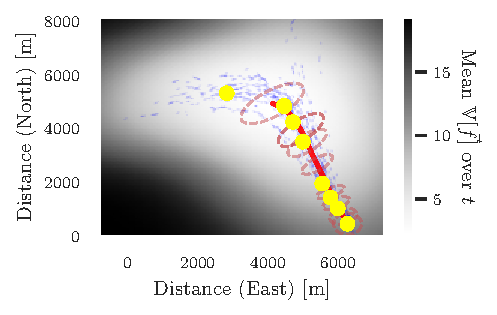
\includegraphics{figures/curved_examples/run_28_pos_no_pdaf.pdf}
            \end{subfigure}
            \begin{subfigure}{.60\textwidth}
                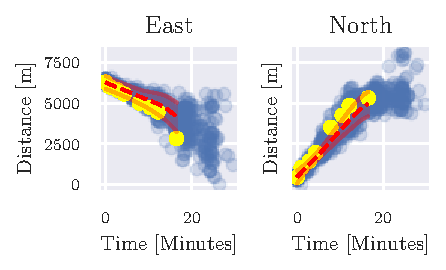
\includegraphics{figures/curved_examples/run_28_state_no_pdaf.pdf}
            \end{subfigure}
        }
        \caption{Basic GP-EKF}
    \end{subfigure}
    \begin{subfigure}{\textwidth}

        \makebox[\textwidth][c] {
            \begin{subfigure}{.65\textwidth}
                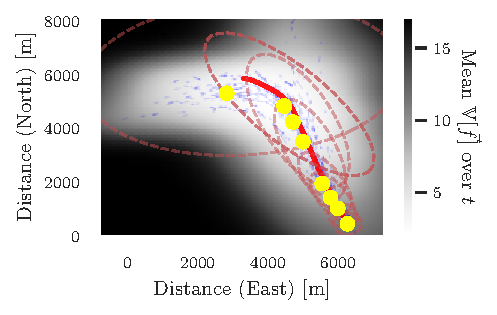
\includegraphics{figures/curved_examples/run_28_pos_no_pdaf_cog.pdf}
            \end{subfigure}
            \begin{subfigure}{.60\textwidth}
                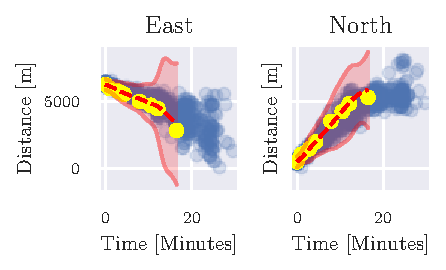
\includegraphics{figures/curved_examples/run_28_state_no_pdaf_cog.pdf}
            \end{subfigure}
        }
        \caption{GP-EKF using \acrshort{cog} / \acrshort{sog} data}
    \end{subfigure}

    \begin{subfigure}{\textwidth}
        \makebox[\textwidth][c] {
            \begin{subfigure}{.65\textwidth}
                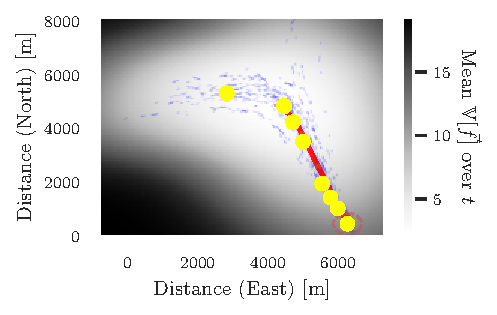
\includegraphics{figures/curved_examples/run_28_pos_pdaf.pdf}
            \end{subfigure}
            \begin{subfigure}{.60\textwidth}
                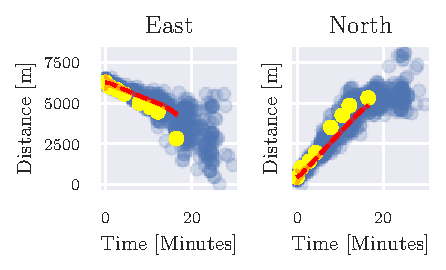
\includegraphics{figures/curved_examples/run_28_state_pdaf.pdf}
            \end{subfigure}
        }
        \caption{GP-EKF With PDAF update}
    \end{subfigure}

    \begin{subfigure}{\textwidth}
        \makebox[\textwidth][c] {
            \begin{subfigure}{.65\textwidth}
                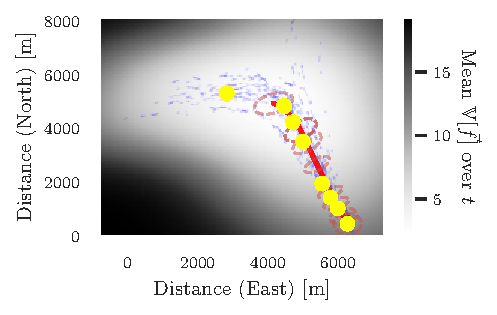
\includegraphics{figures/curved_examples/run_28_pos_syn.pdf}
            \end{subfigure}
            \begin{subfigure}{.60\textwidth}
                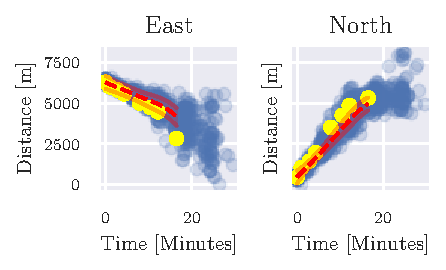
\includegraphics{figures/curved_examples/run_28_state_syn.pdf}
            \end{subfigure}
        }
        \caption{GP-EKF with \acrshort{sl} update}
    \end{subfigure}
    \caption{Case 3}
\end{figure}

\begin{figure}
    \begin{subfigure}{\textwidth}
        \makebox[\textwidth][c] {
            \begin{subfigure}{.65\textwidth}
                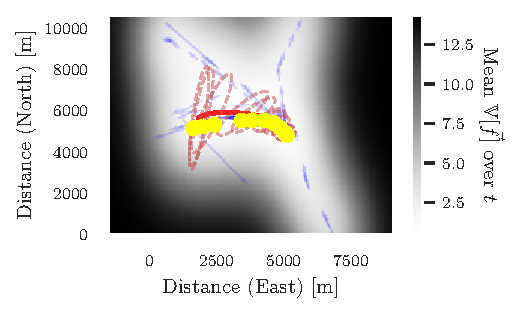
\includegraphics{figures/curved_examples/run_41_pos_no_pdaf.pdf}
            \end{subfigure}
            \begin{subfigure}{.60\textwidth}
                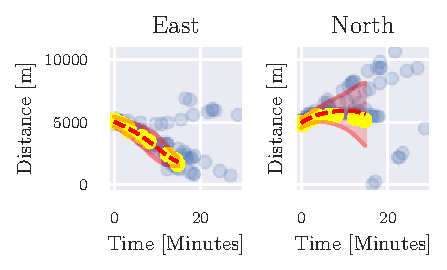
\includegraphics{figures/curved_examples/run_41_state_no_pdaf.pdf}
            \end{subfigure}
        }
        \caption{Basic GP-EKF}
    \end{subfigure}
    \begin{subfigure}{\textwidth}

        \makebox[\textwidth][c] {
            \begin{subfigure}{.65\textwidth}
                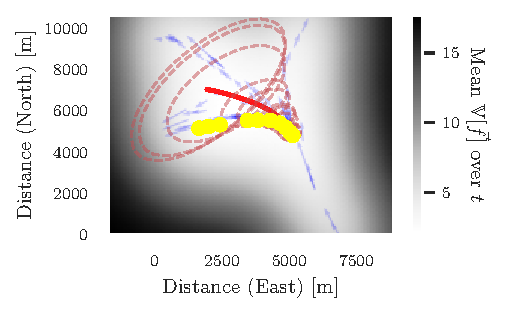
\includegraphics{figures/curved_examples/run_41_pos_no_pdaf_cog.pdf}
            \end{subfigure}
            \begin{subfigure}{.60\textwidth}
                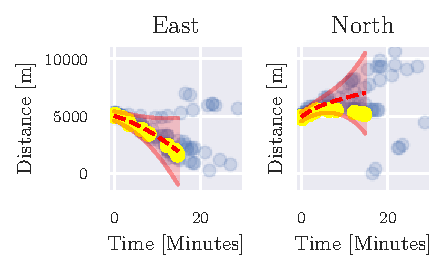
\includegraphics{figures/curved_examples/run_41_state_no_pdaf_cog.pdf}
            \end{subfigure}
        }
        \caption{GP-EKF using \acrshort{cog} / \acrshort{sog} data}
    \end{subfigure}

    \begin{subfigure}{\textwidth}
        \makebox[\textwidth][c] {
            \begin{subfigure}{.65\textwidth}
                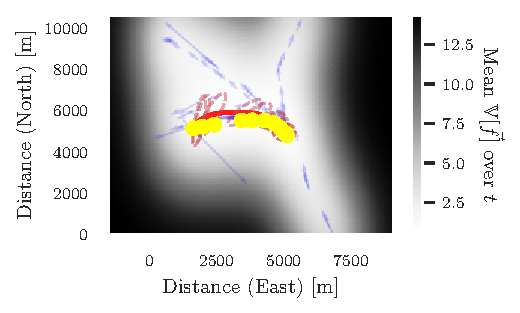
\includegraphics{figures/curved_examples/run_41_pos_pdaf.pdf}
            \end{subfigure}
            \begin{subfigure}{.60\textwidth}
                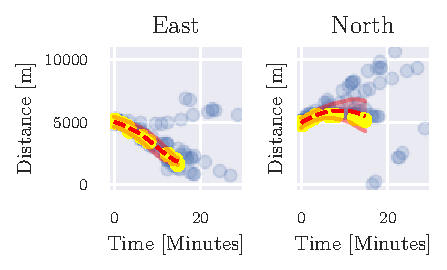
\includegraphics{figures/curved_examples/run_41_state_pdaf.pdf}
            \end{subfigure}
        }
        \caption{GP-EKF With PDAF update}
    \end{subfigure}

    \begin{subfigure}{\textwidth}
        \makebox[\textwidth][c] {
            \begin{subfigure}{.65\textwidth}
                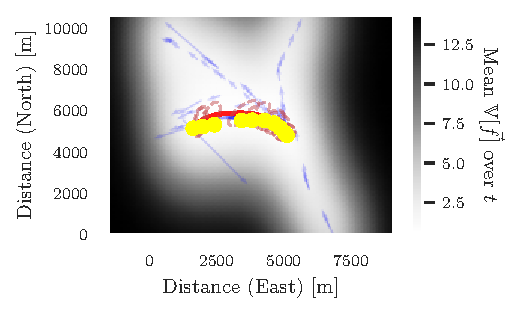
\includegraphics{figures/curved_examples/run_41_pos_syn.pdf}
            \end{subfigure}
            \begin{subfigure}{.60\textwidth}
                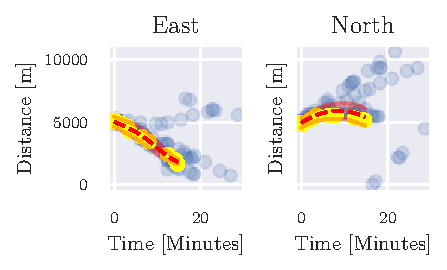
\includegraphics{figures/curved_examples/run_41_state_syn.pdf}
            \end{subfigure}
        }
        \caption{GP-EKF with \acrshort{sl} update}
    \end{subfigure}
    \caption{Case 4}
\end{figure}
\begin{figure}
    \begin{subfigure}{\textwidth}
        \makebox[\textwidth][c] {
            \begin{subfigure}{.65\textwidth}
                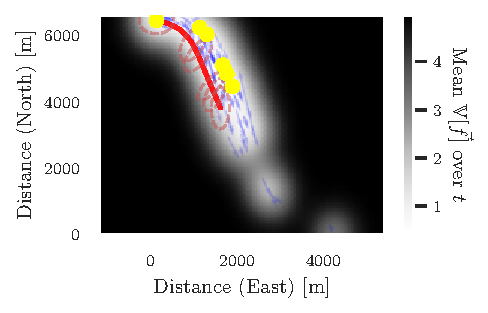
\includegraphics{figures/curved_examples/run_57_pos_no_pdaf.pdf}
            \end{subfigure}
            \begin{subfigure}{.60\textwidth}
                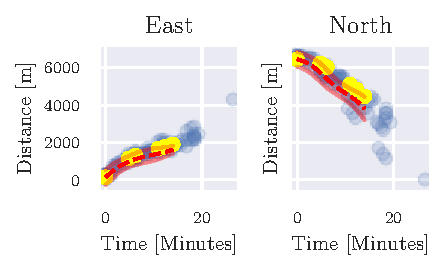
\includegraphics{figures/curved_examples/run_57_state_no_pdaf.pdf}
            \end{subfigure}
        }
        \caption{Basic GP-EKF}
    \end{subfigure}
    \begin{subfigure}{\textwidth}

        \makebox[\textwidth][c] {
            \begin{subfigure}{.65\textwidth}
                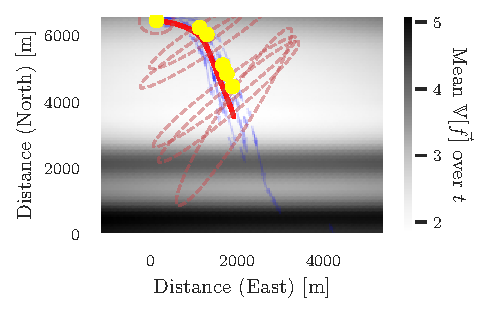
\includegraphics{figures/curved_examples/run_57_pos_no_pdaf_cog.pdf}
            \end{subfigure}
            \begin{subfigure}{.60\textwidth}
                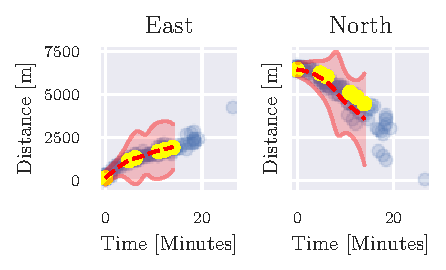
\includegraphics{figures/curved_examples/run_57_state_no_pdaf_cog.pdf}
            \end{subfigure}
        }
        \caption{GP-EKF using \acrshort{cog} / \acrshort{sog} data}
    \end{subfigure}

    \begin{subfigure}{\textwidth}
        \makebox[\textwidth][c] {
            \begin{subfigure}{.65\textwidth}
                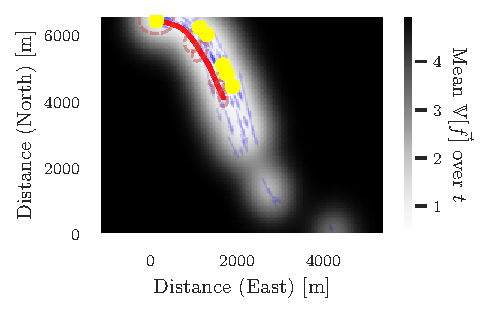
\includegraphics{figures/curved_examples/run_57_pos_pdaf.pdf}
            \end{subfigure}
            \begin{subfigure}{.60\textwidth}
                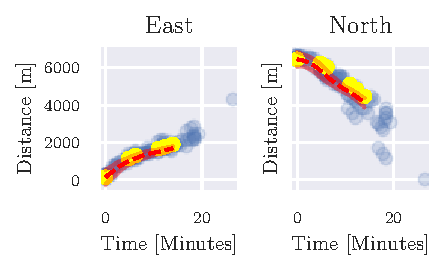
\includegraphics{figures/curved_examples/run_57_state_pdaf.pdf}
            \end{subfigure}
        }
        \caption{GP-EKF With PDAF update}
    \end{subfigure}

    \begin{subfigure}{\textwidth}
        \makebox[\textwidth][c] {
            \begin{subfigure}{.65\textwidth}
                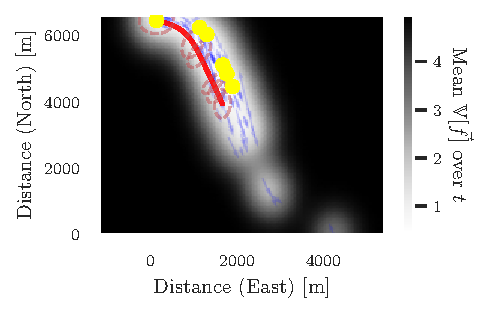
\includegraphics{figures/curved_examples/run_57_pos_syn.pdf}
            \end{subfigure}
            \begin{subfigure}{.60\textwidth}
                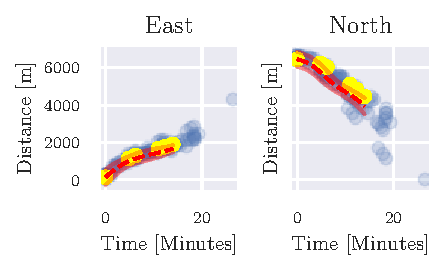
\includegraphics{figures/curved_examples/run_57_state_syn.pdf}
            \end{subfigure}
        }
        \caption{GP-EKF with \acrshort{sl} update}
    \end{subfigure}
    \caption{Case 5}
\end{figure}

\begin{figure}
    \begin{subfigure}{\textwidth}
        \makebox[\textwidth][c] {
            \begin{subfigure}{.65\textwidth}
                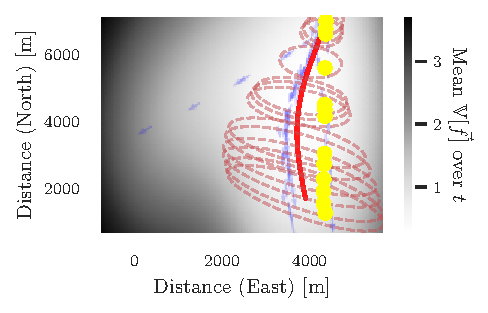
\includegraphics{figures/straight_line_examples/run_28_pos_no_pdaf.pdf}
            \end{subfigure}
            \begin{subfigure}{.60\textwidth}
                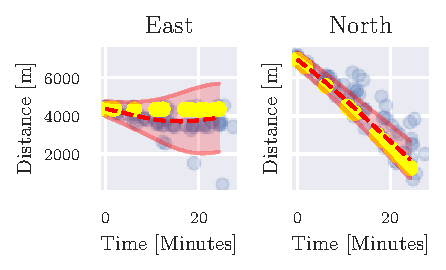
\includegraphics{figures/straight_line_examples/run_28_state_no_pdaf.pdf}
            \end{subfigure}
        }
        \caption{Basic GP-EKF}
    \end{subfigure}
    \begin{subfigure}{\textwidth}

        \makebox[\textwidth][c] {
            \begin{subfigure}{.65\textwidth}
                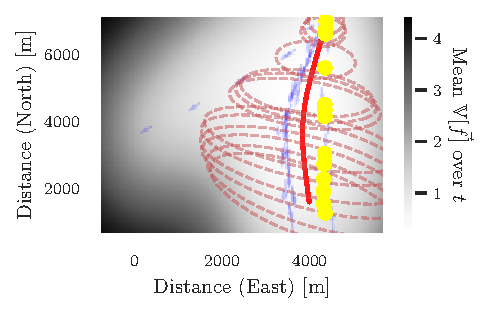
\includegraphics{figures/straight_line_examples/run_28_pos_no_pdaf_cog.pdf}
            \end{subfigure}
            \begin{subfigure}{.60\textwidth}
                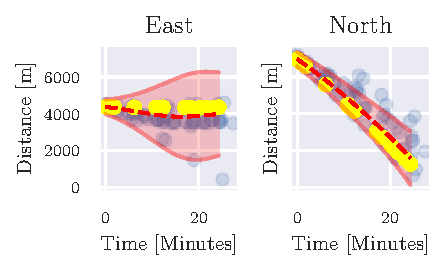
\includegraphics{figures/straight_line_examples/run_28_state_no_pdaf_cog.pdf}
            \end{subfigure}
        }
        \caption{GP-EKF using \acrshort{cog} / \acrshort{sog} data}
    \end{subfigure}

    \begin{subfigure}{\textwidth}
        \makebox[\textwidth][c] {
            \begin{subfigure}{.65\textwidth}
                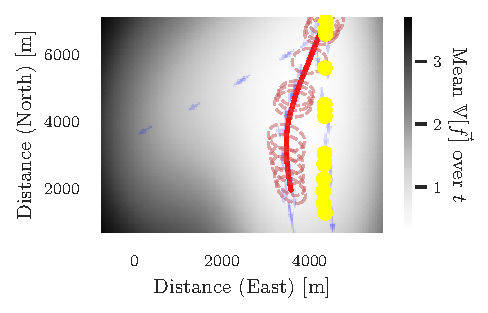
\includegraphics{figures/straight_line_examples/run_28_pos_pdaf.pdf}
            \end{subfigure}
            \begin{subfigure}{.60\textwidth}
                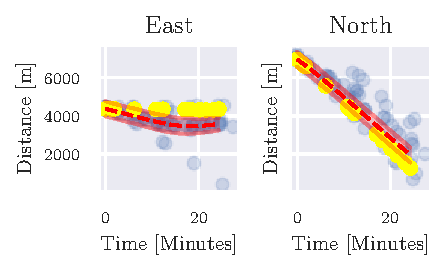
\includegraphics{figures/straight_line_examples/run_28_state_pdaf.pdf}
            \end{subfigure}
        }
        \caption{GP-EKF With PDAF update}
    \end{subfigure}

    \begin{subfigure}{\textwidth}
        \makebox[\textwidth][c] {
            \begin{subfigure}{.65\textwidth}
                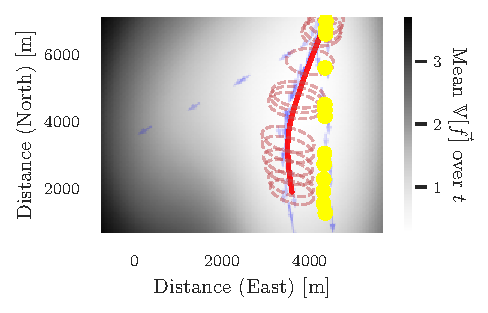
\includegraphics{figures/straight_line_examples/run_28_pos_syn.pdf}
            \end{subfigure}
            \begin{subfigure}{.60\textwidth}
                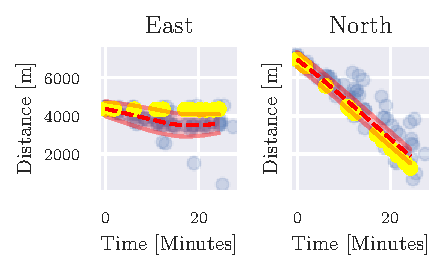
\includegraphics{figures/straight_line_examples/run_28_state_syn.pdf}
            \end{subfigure}
        }
        \caption{GP-EKF with \acrshort{sl} update}
    \end{subfigure}
    \caption{Case 6: Notice how the \acrshort{pdaf} and \acrshort{sl} helps the GP-EKF select a single branch, insteading getting stuck in the middle.}
    \label{fig:app_branching_gp_ekf_update}
\end{figure}

\begin{figure}
    \begin{subfigure}{\textwidth}
        \makebox[\textwidth][c] {
            \begin{subfigure}{.65\textwidth}
                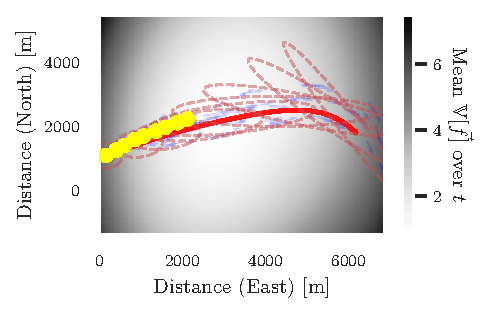
\includegraphics{figures/straight_line_examples/run_32_pos_no_pdaf.pdf}
            \end{subfigure}
            \begin{subfigure}{.60\textwidth}
                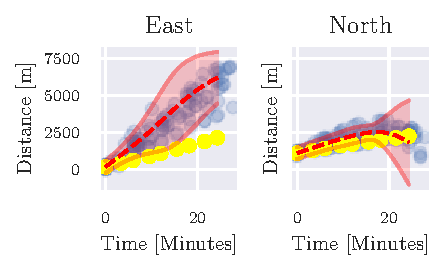
\includegraphics{figures/straight_line_examples/run_32_state_no_pdaf.pdf}
            \end{subfigure}
        }
        \caption{Basic GP-EKF}
    \end{subfigure}
    \begin{subfigure}{\textwidth}

        \makebox[\textwidth][c] {
            \begin{subfigure}{.65\textwidth}
                \includegraphics{figures/straight_line_examples/run_32_pos_no_pdaf_cog.pdf}
            \end{subfigure}
            \begin{subfigure}{.60\textwidth}
                \includegraphics{figures/straight_line_examples/run_32_state_no_pdaf_cog.pdf}
            \end{subfigure}
        }
        \caption{GP-EKF using \acrshort{cog} / \acrshort{sog} data}
    \end{subfigure}

    \begin{subfigure}{\textwidth}
        \makebox[\textwidth][c] {
            \begin{subfigure}{.65\textwidth}
                \includegraphics{figures/straight_line_examples/run_32_pos_pdaf.pdf}
            \end{subfigure}
            \begin{subfigure}{.60\textwidth}
                \includegraphics{figures/straight_line_examples/run_32_state_pdaf.pdf}
            \end{subfigure}
        }
        \caption{GP-EKF With PDAF update}
    \end{subfigure}

    \begin{subfigure}{\textwidth}
        \makebox[\textwidth][c] {
            \begin{subfigure}{.65\textwidth}
                \includegraphics{figures/straight_line_examples/run_32_pos_syn.pdf}
            \end{subfigure}
            \begin{subfigure}{.60\textwidth}
                \includegraphics{figures/straight_line_examples/run_32_state_syn.pdf}
            \end{subfigure}
        }
        \caption{GP-EKF with \acrshort{sl} update}
    \end{subfigure}
    \caption{Case 7: Notice how the training data contains faster vessels, making the GP-EKF overestimate the true velocity.}
\end{figure}

\begin{figure}
    \begin{subfigure}{\textwidth}
        \makebox[\textwidth][c] {
            \begin{subfigure}{.65\textwidth}
                \includegraphics{figures/straight_line_examples/run_61_pos_no_pdaf.pdf}
            \end{subfigure}
            \begin{subfigure}{.60\textwidth}
                \includegraphics{figures/straight_line_examples/run_61_state_no_pdaf.pdf}
            \end{subfigure}
        }
        \caption{Basic GP-EKF}
    \end{subfigure}
    \begin{subfigure}{\textwidth}

        \makebox[\textwidth][c] {
            \begin{subfigure}{.65\textwidth}
                \includegraphics{figures/straight_line_examples/run_61_pos_no_pdaf_cog.pdf}
            \end{subfigure}
            \begin{subfigure}{.60\textwidth}
                \includegraphics{figures/straight_line_examples/run_32_state_no_pdaf_cog.pdf}
            \end{subfigure}
        }
        \caption{GP-EKF using \acrshort{cog} / \acrshort{sog} data}
    \end{subfigure}

    \begin{subfigure}{\textwidth}
        \makebox[\textwidth][c] {
            \begin{subfigure}{.65\textwidth}
                \includegraphics{figures/straight_line_examples/run_61_pos_pdaf.pdf}
            \end{subfigure}
            \begin{subfigure}{.60\textwidth}
                \includegraphics{figures/straight_line_examples/run_61_state_pdaf.pdf}
            \end{subfigure}
        }
        \caption{GP-EKF With PDAF update}
    \end{subfigure}

    \begin{subfigure}{\textwidth}
        \makebox[\textwidth][c] {
            \begin{subfigure}{.65\textwidth}
                \includegraphics{figures/straight_line_examples/run_61_pos_syn.pdf}
            \end{subfigure}
            \begin{subfigure}{.60\textwidth}
                \includegraphics{figures/straight_line_examples/run_61_state_syn.pdf}
            \end{subfigure}
        }
        \caption{GP-EKF with \acrshort{sl} update}
    \end{subfigure}
    \caption{Case 8: Notice how the training data contains faster vessels, making the GP-EKF overestimate the true velocity.}
\end{figure}
